\documentclass[12pt]{scrartcl}

\usepackage[utf8]{inputenc} 
\usepackage[T1]{fontenc}     
\usepackage[french]{babel} 
\usepackage{lmodern}
\usepackage{microtype}
\usepackage{xcolor}
\usepackage{sectsty}
\usepackage{geometry} 
\usepackage{fancyhdr}  
\usepackage{graphicx}        
\usepackage{amsmath, amssymb} 
\usepackage[hidelinks]{hyperref} 

\hypersetup{pdfnewwindow=true}
\setcounter{secnumdepth}{0}   
\definecolor{mainblue}{RGB}{0, 102, 204}
\sectionfont{\color{blue!60!black}\sffamily\Large\bfseries}  
\geometry{margin=2cm}


%%%%%%%%%%%%%%%%%%%%%%%%%%%%%%%%%%%%%%%%%%%%%%%%%%%%%%%%%%%%%%%%%%%%%%%%%%%%%%%%%%%%%%%
%%%%%%%%%%                       EN-TÊTE ET PIED DE PAGE                     %%%%%%%%%%
%%%%%%%%%%%%%%%%%%%%%%%%%%%%%%%%%%%%%%%%%%%%%%%%%%%%%%%%%%%%%%%%%%%%%%%%%%%%%%%%%%%%%%%

\pagestyle{fancy}
\fancyhf{} 

%%% En-tête de page
\fancyhead[L]{\footnotesize IUT de Lannion - Département Informatique}
\fancyhead[R]{\footnotesize 2025} 

%%% Pied de page
\fancyfoot[L]{\footnotesize © Stanislas ROLLAND - Pierre LECHAT - Tous droits réservés} 
\fancyfoot[R]{\footnotesize \thepage}

\renewcommand{\footrulewidth}{0.4pt}


%%%%%%%%%%%%%%%%%%%%%%%%%%%%%%%%%%%%%%%%%%%%%%%%%%%%%%%%%%%%%%%%%%%%%%%%%%%%%%%%%%%%%%%
%%%%%%%%%%                        PAGE DE PRÉSENTATION                       %%%%%%%%%%
%%%%%%%%%%%%%%%%%%%%%%%%%%%%%%%%%%%%%%%%%%%%%%%%%%%%%%%%%%%%%%%%%%%%%%%%%%%%%%%%%%%%%%%

\title{RAPPORT D'ANALYSE DE DONNÉES}
\author{Stanislas ROLLAND - Pierre LECHAT}
\date{Septembre 2025}

\begin{document}

    \maketitle
    \tableofcontents  
    \newpage
 

    %%%%%%%%%%%%%%%%%%%%%%%%%%%%%%%%%%%%%%%%%%%%%%%%%%%%%%%%%%%%%%%%%%%%%%%%%%%%%%%%%%%
    %%%%%%%%%%                          INTRODUCTION                         %%%%%%%%%%
    %%%%%%%%%%%%%%%%%%%%%%%%%%%%%%%%%%%%%%%%%%%%%%%%%%%%%%%%%%%%%%%%%%%%%%%%%%%%%%%%%%%

    \section{Introduction}

        Dans le cadre de notre formation en BUT Informatique à l'IUT de Lannion, nous avons été amenés à réaliser un projet d'analyse de données.\\\\
        Nous avons choisi d'analyser un jeu de données concernant les statistiques des joueurs de football évoluant dans les cinq meilleures ligues européennes durant la saison 2024 - 2025. Ce choix a été motivé par notre intérêt commun pour le football et par la richesse des données disponibles dans ce domaine.\\\\
        Le présent rapport détaille les différentes étapes de notre analyse, depuis la présentation du jeu de données jusqu'aux techniques d'analyse utilisées, en passant par les résultats obtenus et leur interprétation.


    %%%%%%%%%%%%%%%%%%%%%%%%%%%%%%%%%%%%%%%%%%%%%%%%%%%%%%%%%%%%%%%%%%%%%%%%%%%%%%%%%%%
    %%%%%%%%%%                         JEU DE DONNÉES                        %%%%%%%%%%
    %%%%%%%%%%%%%%%%%%%%%%%%%%%%%%%%%%%%%%%%%%%%%%%%%%%%%%%%%%%%%%%%%%%%%%%%%%%%%%%%%%%

    \section{Présentation du jeu de données}

        \subsection{Description du jeu de données}
            Le jeu de données que nous avons choisi d'analyser est un ensemble de données concernant les statistiques des joueurs de football sur la saison 2024 - 2025 les cinq meilleures ligues européennes (Premier League, La Liga, Serie A, Ligue 1, Bundesliga).\\\\
            Notre jeu de données comporte 197 entrées (une par joueur) et les 15 variables suivantes :

            \textbf{\\\underline{Variables qualitatives :}\\}
                \begin{itemize}
                    \item \textbf{Player} : Nom et prénom du joueur.
                    \item \textbf{Nation} : Nationalité du joueur.
                    \item \textbf{Pos} : Position principale du joueur sur le terrain (ex : Attaquant, Défenseur, Gardien).
                    \item \textbf{Squad} : Équipe actuelle du joueur.
                    \item \textbf{Comp} : Compétition dans laquelle le joueur évolue (ex : Premier League, La Liga etc).
                \end{itemize}
            
            \textbf{\\\underline{Variables quantitatives :}\\}
                \begin{itemize}
                    \item \textbf{Id} : Identifiant unique du joueur.
                    \item \textbf{Age} : Âge du joueur.
                    \item \textbf{Born} : Année de naissance du joueur.
                    \item \textbf{MP} : Nombre de matchs joués par le joueur.
                    \item \textbf{Starts} : Nombre de matchs commencés comme titulaire.
                    \item \textbf{Min} : Nombre total de minutes jouées.
                    \item \textbf{90s} : Nombre de périodes de 90 minutes jouées (équivalent à des matchs complets).
                    \item \textbf{Gls} : Nombre total de buts marqués.
                    \item \textbf{Ast} : Nombre total de passes décisives.
                    \item \textbf{G+A} : Somme des buts et des passes décisives.
                \end{itemize}

        \subsection{Exemple d'une entrée du jeu de données}

            \begin{center}
                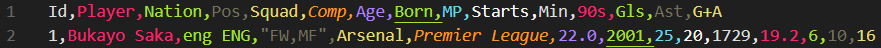
\includegraphics[width=1\textwidth]{images/exemple_entree.png}
                \captionof{figure}{}
            \end{center}    


    %%%%%%%%%%%%%%%%%%%%%%%%%%%%%%%%%%%%%%%%%%%%%%%%%%%%%%%%%%%%%%%%%%%%%%%%%%%%%%%%%%%
    %%%%%%%%%%               TECHNIQUES D'ANALYSE DE DONNÉES                 %%%%%%%%%%
    %%%%%%%%%%%%%%%%%%%%%%%%%%%%%%%%%%%%%%%%%%%%%%%%%%%%%%%%%%%%%%%%%%%%%%%%%%%%%%%%%%%

    \section{Présentation des techniques d'analyse de données}


    %%%%%%%%%%%%%%%%%%%%%%%%%%%%%%%%%%%%%%%%%%%%%%%%%%%%%%%%%%%%%%%%%%%%%%%%%%%%%%%%%%%
    %%%%%%%%%%                  ANALYSE QUANTITATIVE : APC                   %%%%%%%%%%
    %%%%%%%%%%%%%%%%%%%%%%%%%%%%%%%%%%%%%%%%%%%%%%%%%%%%%%%%%%%%%%%%%%%%%%%%%%%%%%%%%%%

    \section{Analyse quantitative des données : l'ACP}

        \subsection{Définition}
            L'Analyse en Composantes Principales (ACP) est une technique statistique utilisée pour réduire la dimensionnalité d'un jeu de données tout en conservant le maximum d'information possible. Elle permet de transformer un ensemble de variables corrélées en un ensemble de variables non corrélées appelées composantes principales.\\\\
            L'ACP est particulièrement utile lorsque l'on travaille avec des données multivariées, c'est-à-dire des données comportant plusieurs variables quantitatives. En réduisant le nombre de dimensions, l'ACP facilite la visualisation et l'interprétation des données, tout en aidant à identifier les structures sous-jacentes et les relations entre les variables.\\


        %%%%%%%%%%%%%%%%%%%%%%%%%%%%%%%%%%%%%%%%%%%%%%%%%%%%%%%%%%%%%%%%%%%%%%%%%%%%%%%%%%%
        %%%%%%%%%%                     CERCLE DE CORRÉLATION                     %%%%%%%%%%
        %%%%%%%%%%%%%%%%%%%%%%%%%%%%%%%%%%%%%%%%%%%%%%%%%%%%%%%%%%%%%%%%%%%%%%%%%%%%%%%%%%%

        \subsection{Cercle de corrélation}
            \subsubsection{Définition}
                Le cercle de corrélation est un outil graphique utilisé dans le cadre de l'ACP pour visualiser les relations entre les variables originales et les composantes principales. Chaque variable est représentée par un vecteur dans un plan défini par les deux premières composantes principales.\\\\
                La position et la longueur des vecteurs permettent d'interpréter la contribution de chaque variable aux composantes principales. Par exemple, des vecteurs proches les uns des autres indiquent des variables fortement corrélées, tandis que des vecteurs perpendiculaires suggèrent une absence de corrélation. La distance d'un vecteur à l'origine reflète l'importance de la variable dans la formation des composantes principales.\\
                
                \begin{center}
                    \includegraphics[width=1\textwidth]{images/cercle_de_corrélation.png}
                    \captionof{figure}{}
                \end{center}

            \subsubsection{Interprétation}
                Dans la figure ci-dessus, on peut observer que les variables "Gls" et "G+A" sont plus ou moins corréléeses car "G+A" est la somme de "Gls" et "Ast". En revanche la variable "Ast" n'est pas corrélées avec ces dernières, ce qui peut être expliqué par le fait que les joueurs qui inscrivent beaucoup de buts inscrivent généralement beaucoup moins de passes décisives.\\\\
                Quant à elle, les variables "MP", "Starts", "Min" et "90s" sont également fortement corrélées entre elles, ce qui reflète le fait que ces variables mesurent différentes facettes du temps de jeu des joueurs.\\\\
                La variable "Age", elle, semble être très faiblement corrélée avec les autres variables, ce qui peut indiquer que l'âge des joueurs n'a pas une influence directe sur leurs performances statistiques dans ce jeu de données.\\
    

        %%%%%%%%%%%%%%%%%%%%%%%%%%%%%%%%%%%%%%%%%%%%%%%%%%%%%%%%%%%%%%%%%%%%%%%%%%%%%%%%%%%
        %%%%%%%%%%                   GRAPHIQUE DES INDIVIDUS                     %%%%%%%%%%
        %%%%%%%%%%%%%%%%%%%%%%%%%%%%%%%%%%%%%%%%%%%%%%%%%%%%%%%%%%%%%%%%%%%%%%%%%%%%%%%%%%%

        \subsection{Graphique des individus}
            \subsubsection{Définition}
                Le graphique des individus est un outil visuel utilisé dans le cadre de l'ACP pour représenter les observations (individus) dans l'espace défini par les composantes principales. Chaque point sur le graphique correspond à une observation du jeu de données, et la position de chaque point est déterminée par ses coordonnées sur les axes des composantes principales.\\\\
                Ce graphique permet d'identifier des groupes d'individus similaires, des tendances générales, ainsi que des observations atypiques ou des outliers. En analysant la distribution des points, on peut tirer des conclusions sur la structure sous-jacente des données et sur les relations entre les différentes observations.\\

                \begin{center}
                    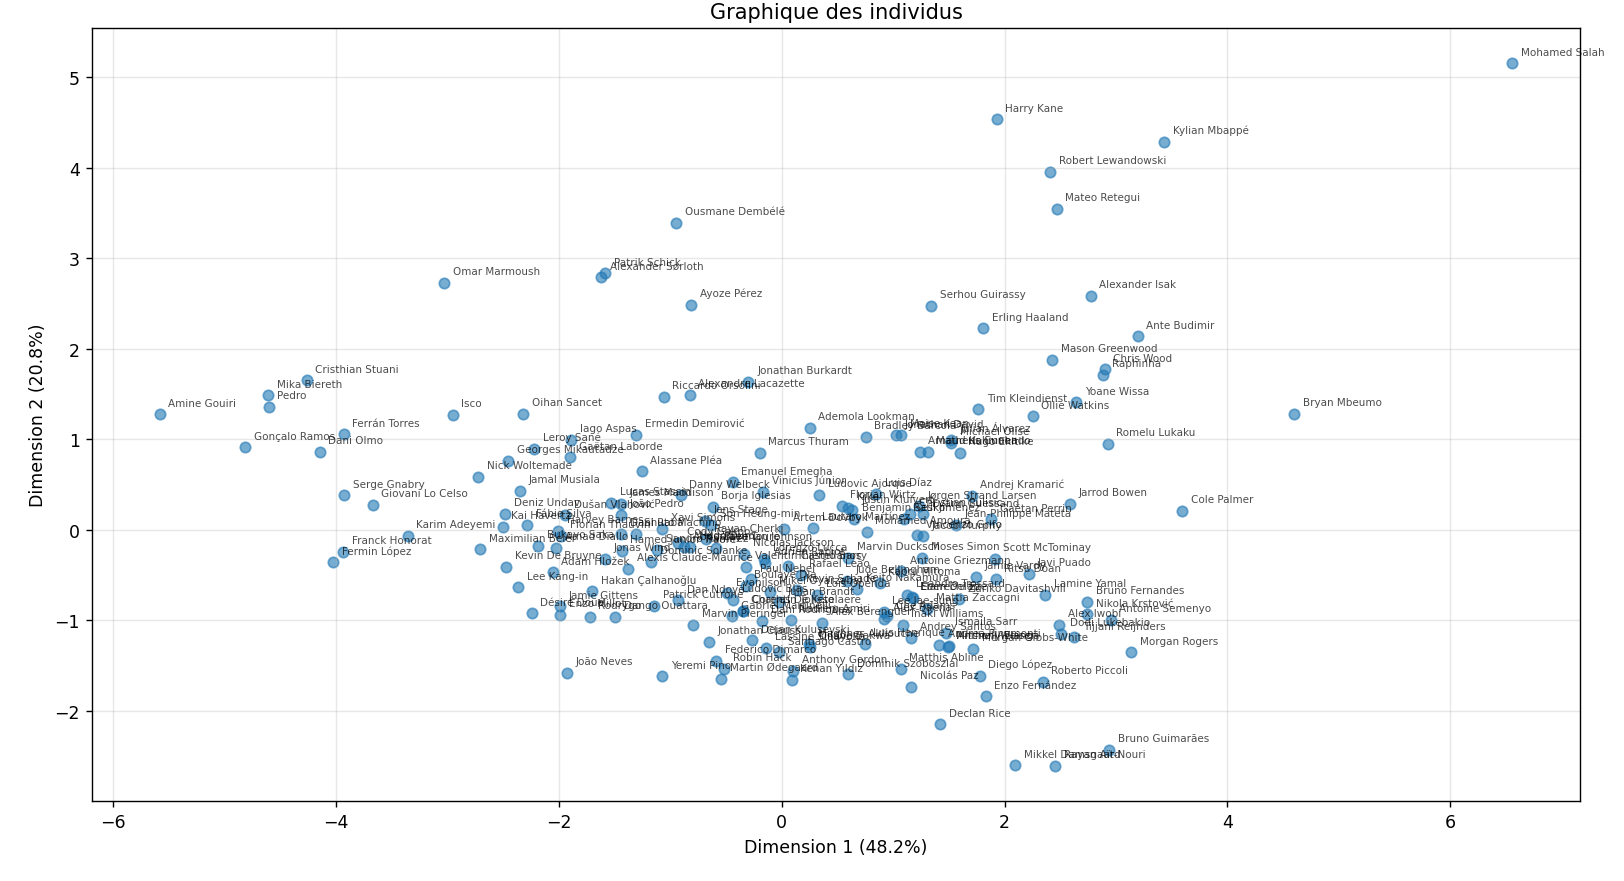
\includegraphics[width=1\textwidth]{images/graphique_des_individus.png}
                    \captionof{figure}{}
                \end{center}

            \subsubsection{Interprétation}
                Dans la figure ci-dessus, on peut observer que les joueurs sont répartis en plusieurs groupes distincts. Par exemple, on peut identifier un groupe de joueurs situés dans la partie supérieure droite du graphique, qui sont probablement des attaquants ou des milieux offensifs, car ils ont des valeurs élevées pour les variables "Gls" et "G+A".\\\\
                En revanche, les joueurs situés dans la partie inférieure gauche du graphique ont des valeurs plus faibles pour ces variables, ce qui suggère qu'ils occupent des postes plus reculés et / ou orientés sur la défense.\\\\
                De plus, on peut remarquer que certains joueurs sont situés loin du centre du graphique, ce qui indique qu'ils ont des performances statistiques atypiques par rapport à la majorité des joueurs. Ces observations peuvent être considérées comme des outliers et méritent une attention particulière pour comprendre les raisons de leurs performances exceptionnelles ou médiocres.\\

                \begin{center}
                    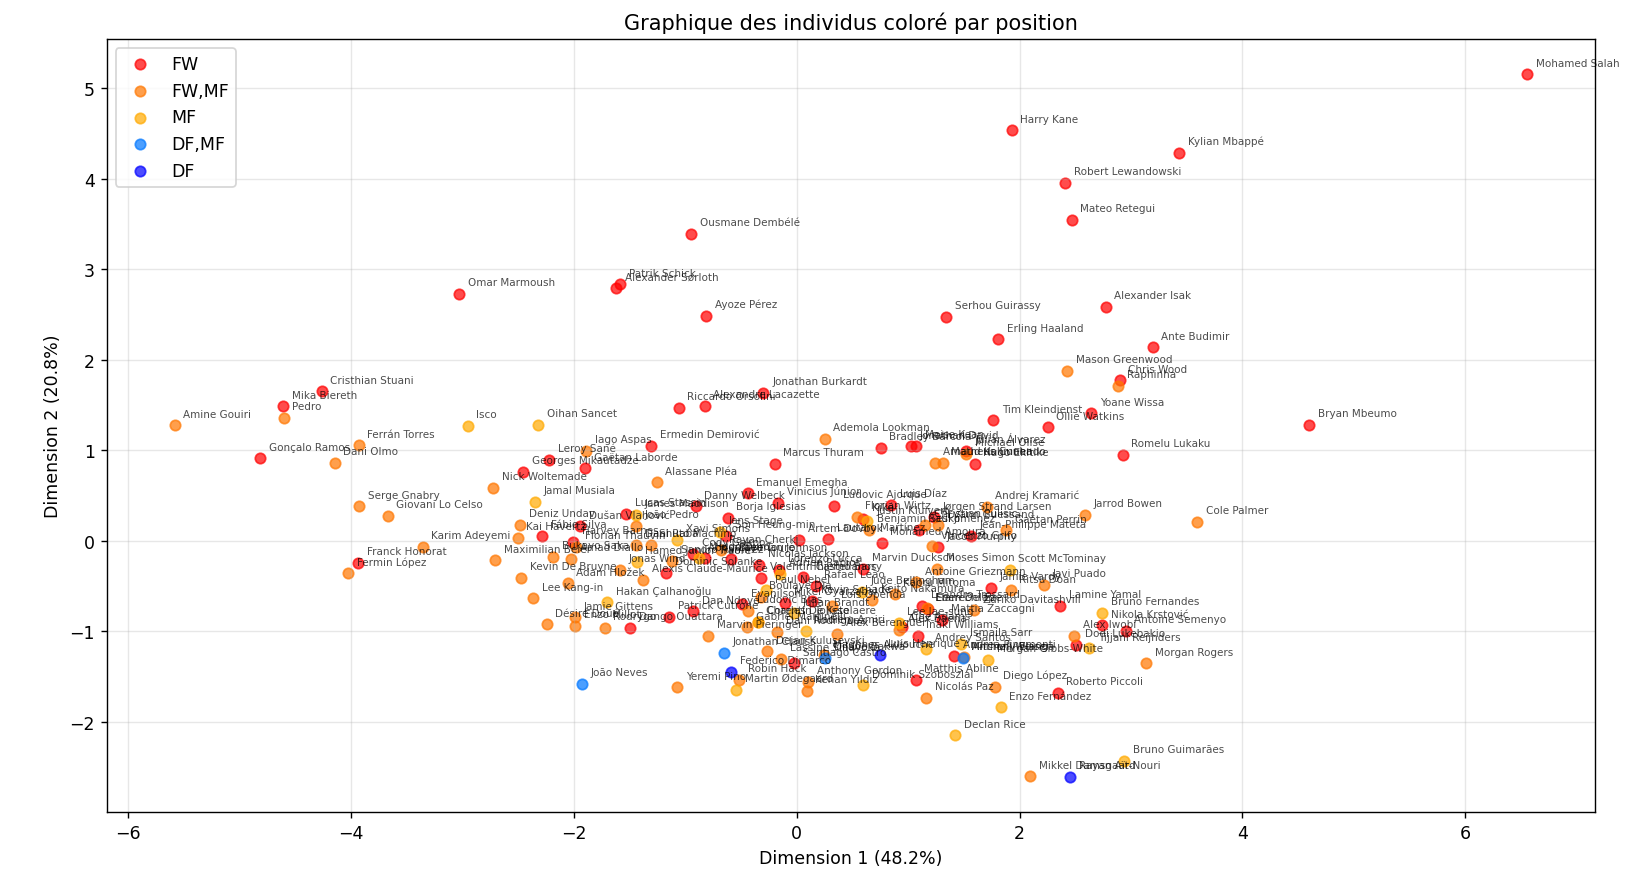
\includegraphics[width=1\textwidth]{images/graphique_des_individus_positions.png}
                    \captionof{figure}{}
                \end{center}

            \subsubsection{Interprétation}
                La figure ci-dessus confirme notre interprétation précédente, en effet, on peut observer que les joueurs représentés par des couleurs chaudes comme le rouge et l'orange se démarquent par rapport aux autres car ils occupent des postes avancés sur le terrain et donc qu'ils inscrivent plus de buts que les joueurs occupant des postes reculés.\\\\
                Les joueurs représentés avec des couleurs plus froides, notamement le bleu foncé, sont situés dans la partie inférieure , ce qui confirme donc que même les meilleurs joueurs occupant des postes reculés inscrivent très peu de buts comparé aux joueurs avec des postes avancés.\\

                \begin{center}
                    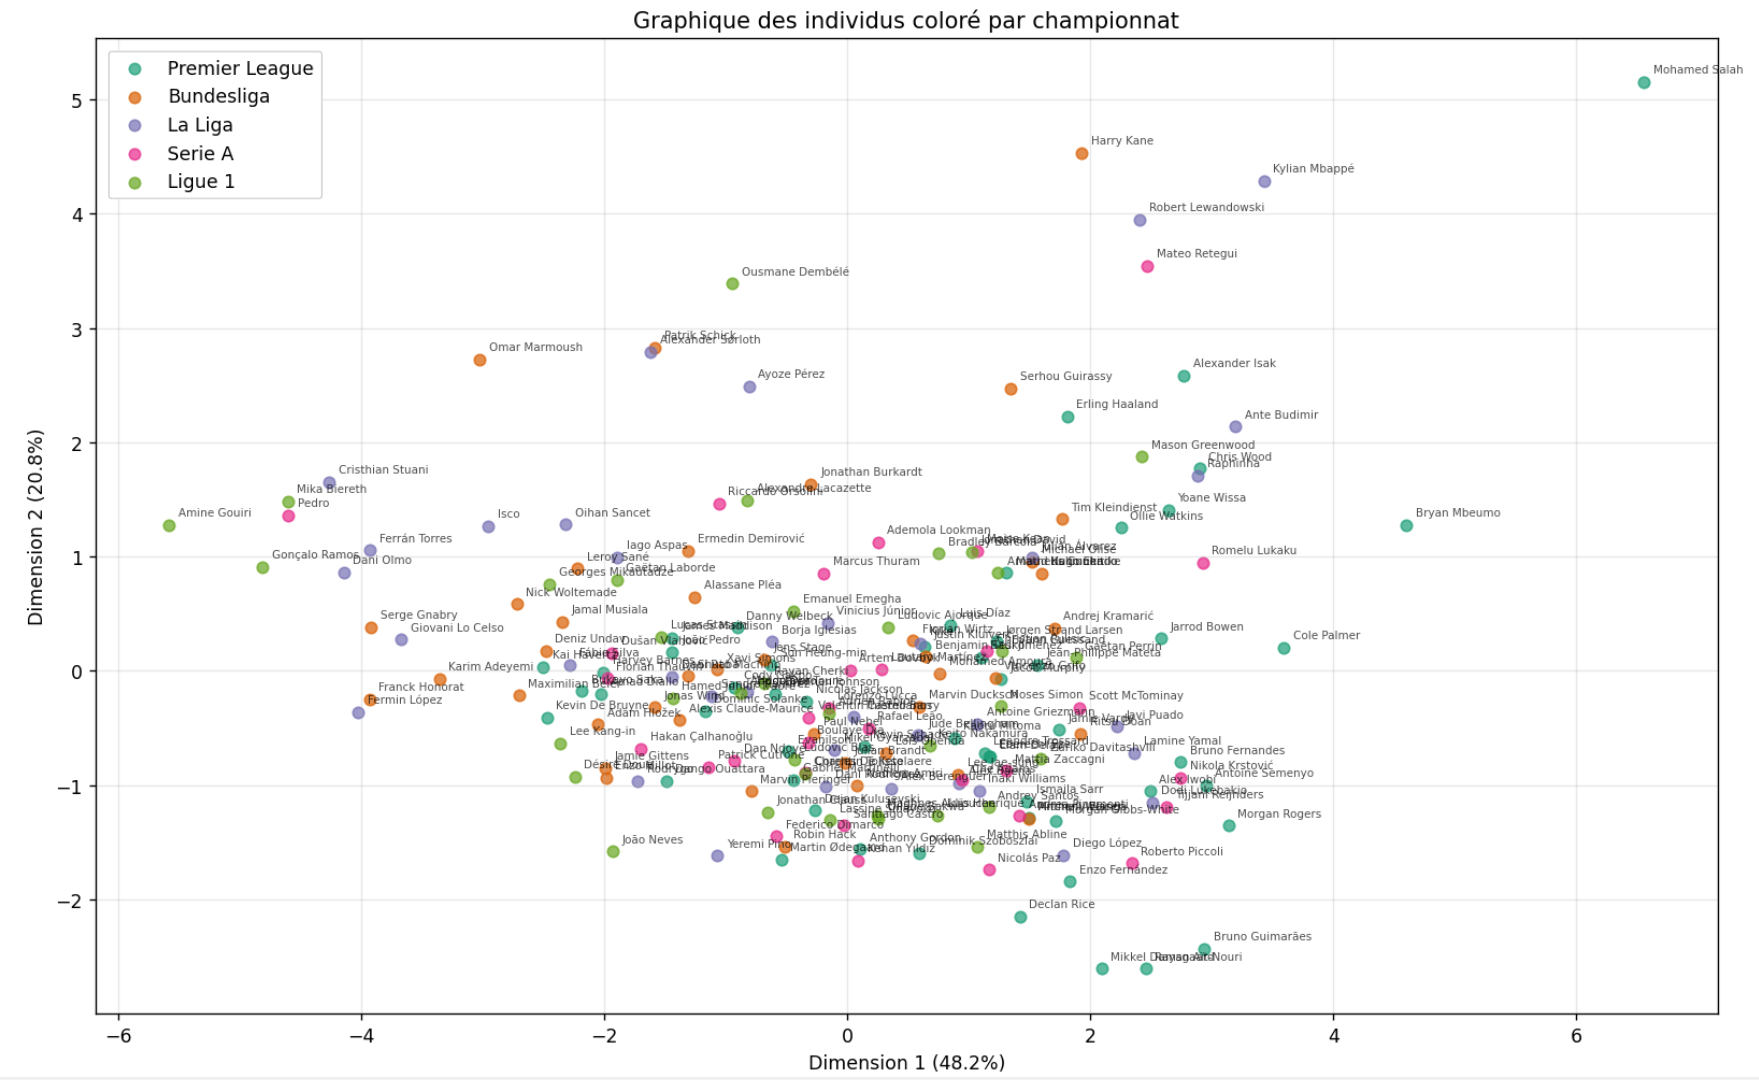
\includegraphics[width=1\textwidth]{images/graphique_des_individus_championnats.png}
                    \captionof{figure}{}
                \end{center}

            \subsubsection{Interprétation}
                Dans la figure ci-dessus, on constate qu'il est difficile de distinguer les joueurs en fonction des championnats dans lesquels ils évoluent. En effet, les joueurs de différents championnats sont dispersés de manière plutôt homogène sur le graphique, ce qui suggère que les performances statistiques des joueurs ne sont pas fortement influencées par le championnat dans lequel ils jouent.\\\\


        %%%%%%%%%%%%%%%%%%%%%%%%%%%%%%%%%%%%%%%%%%%%%%%%%%%%%%%%%%%%%%%%%%%%%%%%%%%%%%%%%%%
        %%%%%%%%%%                        VALEURS PROPRES                        %%%%%%%%%%
        %%%%%%%%%%%%%%%%%%%%%%%%%%%%%%%%%%%%%%%%%%%%%%%%%%%%%%%%%%%%%%%%%%%%%%%%%%%%%%%%%%%

        \subsection{Valeurs propres}
            \subsubsection{Définition}
                Les valeurs propres mesurent l’importance de chaque composante principale dans une ACP. Plus la valeur est grande, plus la composante explique une part importante de la variance des données. À l’inverse, une petite valeur signifie que la composante apporte peu d’information.\\\\
                En général, on retient les composantes principales dont les valeurs propres sont supérieures à 1, car elles expliquent plus de variance qu’une variable originale.\\

                \begin{center}
                    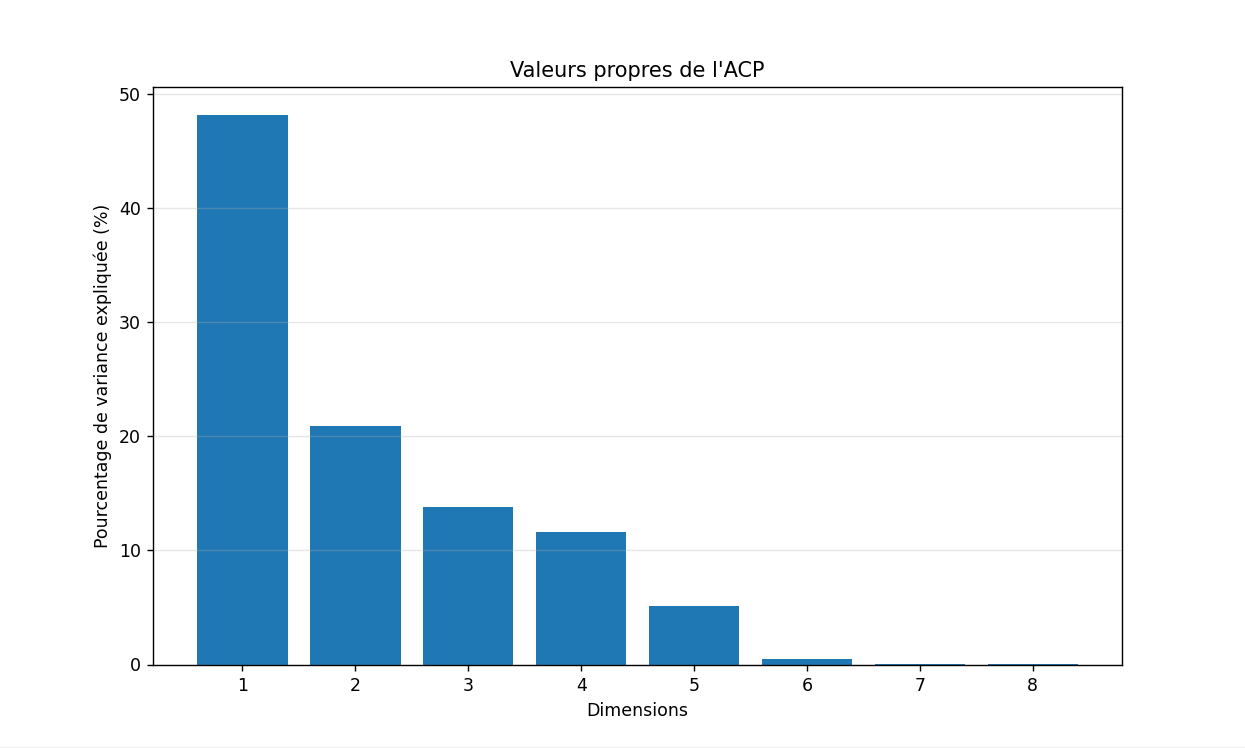
\includegraphics[width=1\textwidth]{images/valeurs_propres_ACP.png}
                    \captionof{figure}{}
                \end{center}

            \subsubsection{Interprétation}
                Dans la figure ci-dessus, on peut observer que les deux premières composantes principales ont des valeurs propres significativement plus élevées que les autres (près de 70\% de la variance totale expliquée). Cela indique que ces deux composantes capturent la majorité de l'information contenue dans les données et donc prouvent que l'ACP réduit efficacement la dimension du jeu de données.\\\\
                Cependant, bien que ces deux premières couvrent la majeure partie du jeu de données, il est préférable de conserver les quatres premières composantes principales pour obtenir une représentation plus fidèle de notre jeu de données (environ 90\%).\\                
            
                
    %%%%%%%%%%%%%%%%%%%%%%%%%%%%%%%%%%%%%%%%%%%%%%%%%%%%%%%%%%%%%%%%%%%%%%%%%%%%%%%%%%%
    %%%%%%%%%%                  ANALYSE CATÉGORIELLE : AFC                   %%%%%%%%%%
    %%%%%%%%%%%%%%%%%%%%%%%%%%%%%%%%%%%%%%%%%%%%%%%%%%%%%%%%%%%%%%%%%%%%%%%%%%%%%%%%%%%
        
    \section{Analyse catégorielle des données : AFC}

        \subsection{Définition}
            L'Analyse Factorielle des Correspondances (AFC) est une technique statistique utilisée pour analyser des données qualitatives, souvent présentées sous forme de tableaux de contingence. Elle permet de visualiser les relations entre les catégories de deux variables qualitatives en les représentant dans un espace à deux dimensions.\\\\
            L'AFC est particulièrement utile pour identifier des associations entre les catégories, détecter des groupes similaires et comprendre la structure sous-jacente des données qualitatives. En réduisant la complexité des données, l'AFC facilite l'interprétation et la communication des résultats.\\


        %%%%%%%%%%%%%%%%%%%%%%%%%%%%%%%%%%%%%%%%%%%%%%%%%%%%%%%%%%%%%%%%%%%%%%%%%%%%%%%%%%%
        %%%%%%%%%%                 GRAPHIQUE DES ASSOCIATIONS                    %%%%%%%%%%
        %%%%%%%%%%%%%%%%%%%%%%%%%%%%%%%%%%%%%%%%%%%%%%%%%%%%%%%%%%%%%%%%%%%%%%%%%%%%%%%%%%%

        \subsection{Graphique des associations}
            \subsubsection{Définition}
                Le graphique des associations est un outil visuel utilisé dans le cadre de l'AFC pour représenter les relations entre les catégories de deux variables qualitatives. Chaque catégorie est représentée par un point dans un plan défini par les deux premières dimensions de l'analyse.\\\\
                Ce graphique permet d'identifier des associations entre les catégories, des tendances générales, ainsi que des groupes similaires. En analysant la distribution des points, on peut tirer des conclusions sur la structure sous-jacente des données et sur les relations entre les différentes catégories.\\

                \begin{center}
                    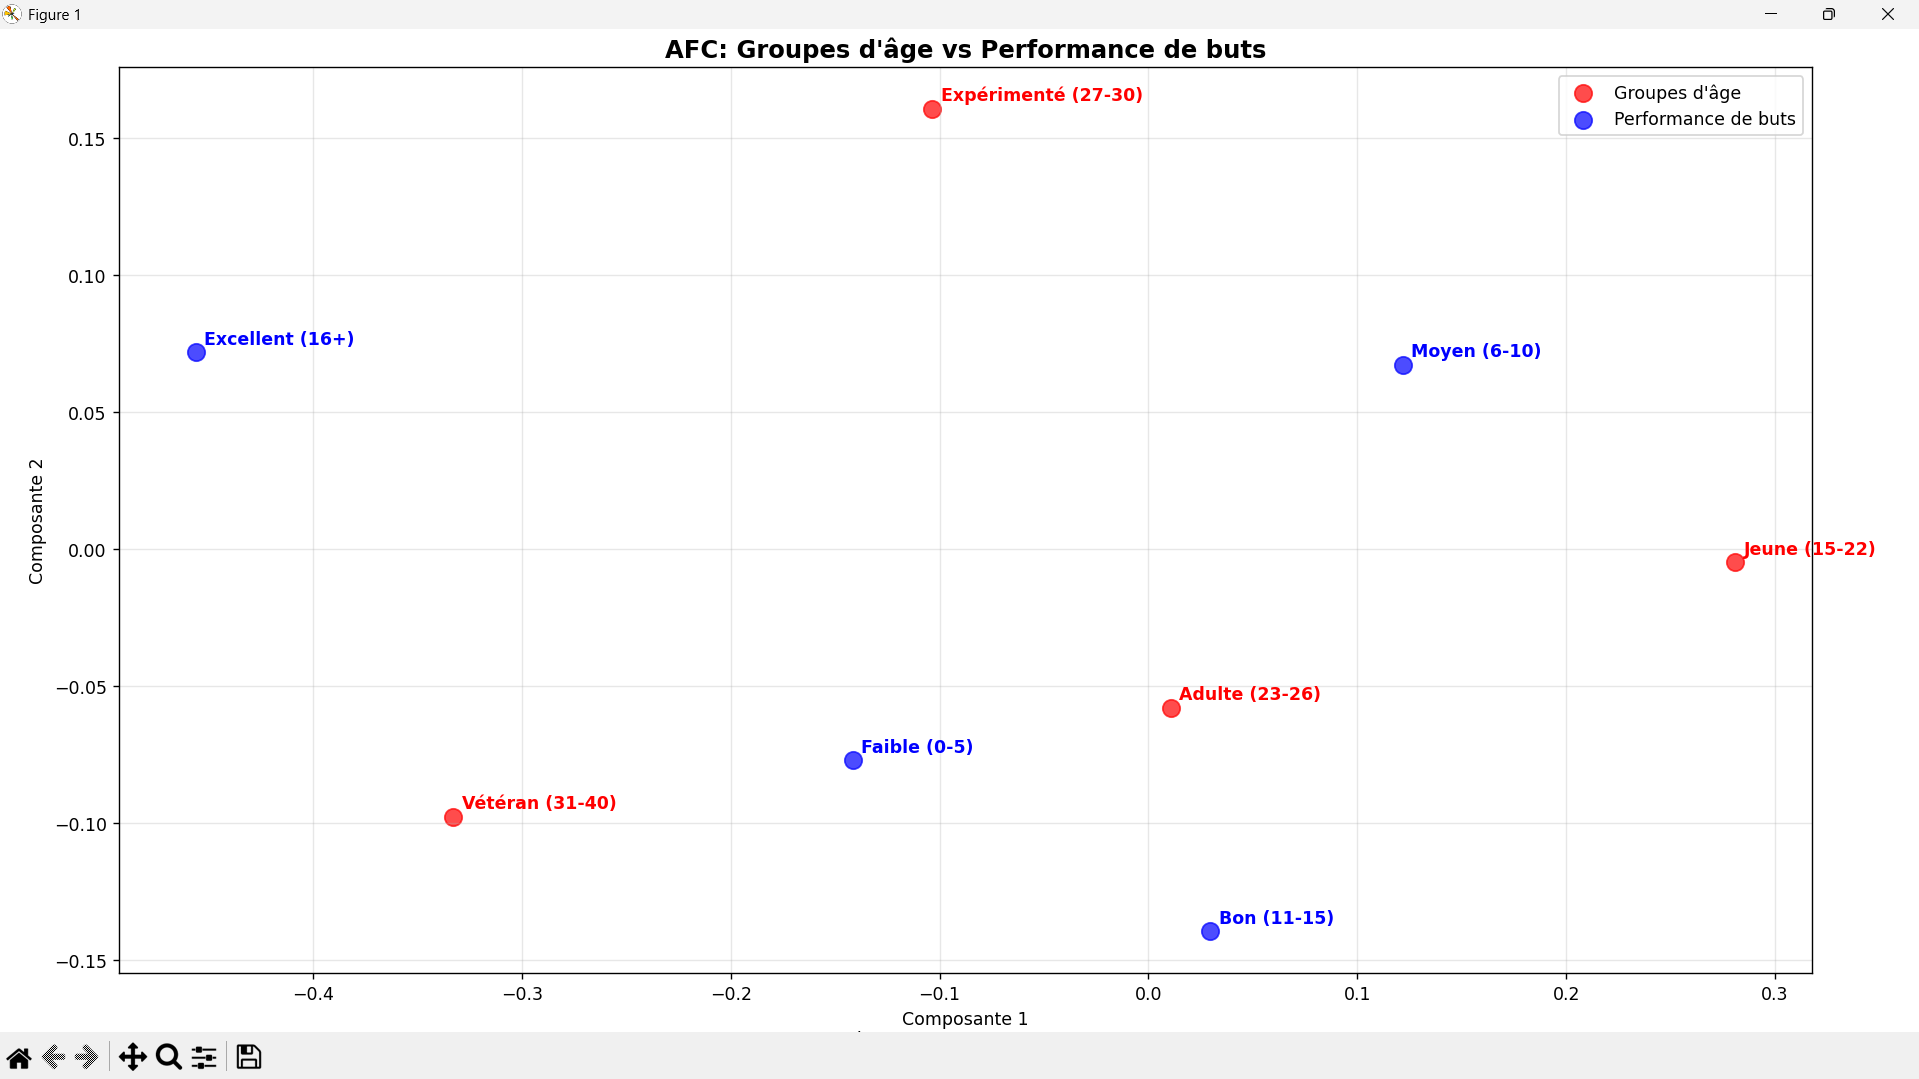
\includegraphics[width=1\textwidth]{images/graphique_AFC_buts.png}
                    \captionof{figure}{}
                \end{center}

            \subsubsection{Interprétation}
                Dans la figure ci-dessus, on peut observer qu'il existe une progression logique des performances en fonction de l’âge. En effet, les joueurs jeunes (15–22 ans) se situent à proximité de la catégorie "Moyen (6–10 buts)", indiquant qu’ils obtiennent généralement des résultats corrects mais encore en phase de progression. Les adultes (23–26 ans) se rapprochent de la catégorie "Bon (11–15 buts)", reflétant une amélioration notable liée à une plus grande expérience de jeu.\\\\
                Les joueurs expérimentés (27–30 ans) se distinguent clairement par leur proximité avec la catégorie "Excellent (16+)", suggérant que cette tranche d’âge correspond au pic de performance dans la carrière des joueurs contrairement aux vétérans (31–40 ans) qui, eux, se trouvent du côté opposé du plan factoriel, proches de la catégorie "Faible (0–5 buts)" ce qui traduit une diminution naturelle et logique des performances avec l’âge.\\

                \begin{center}
                    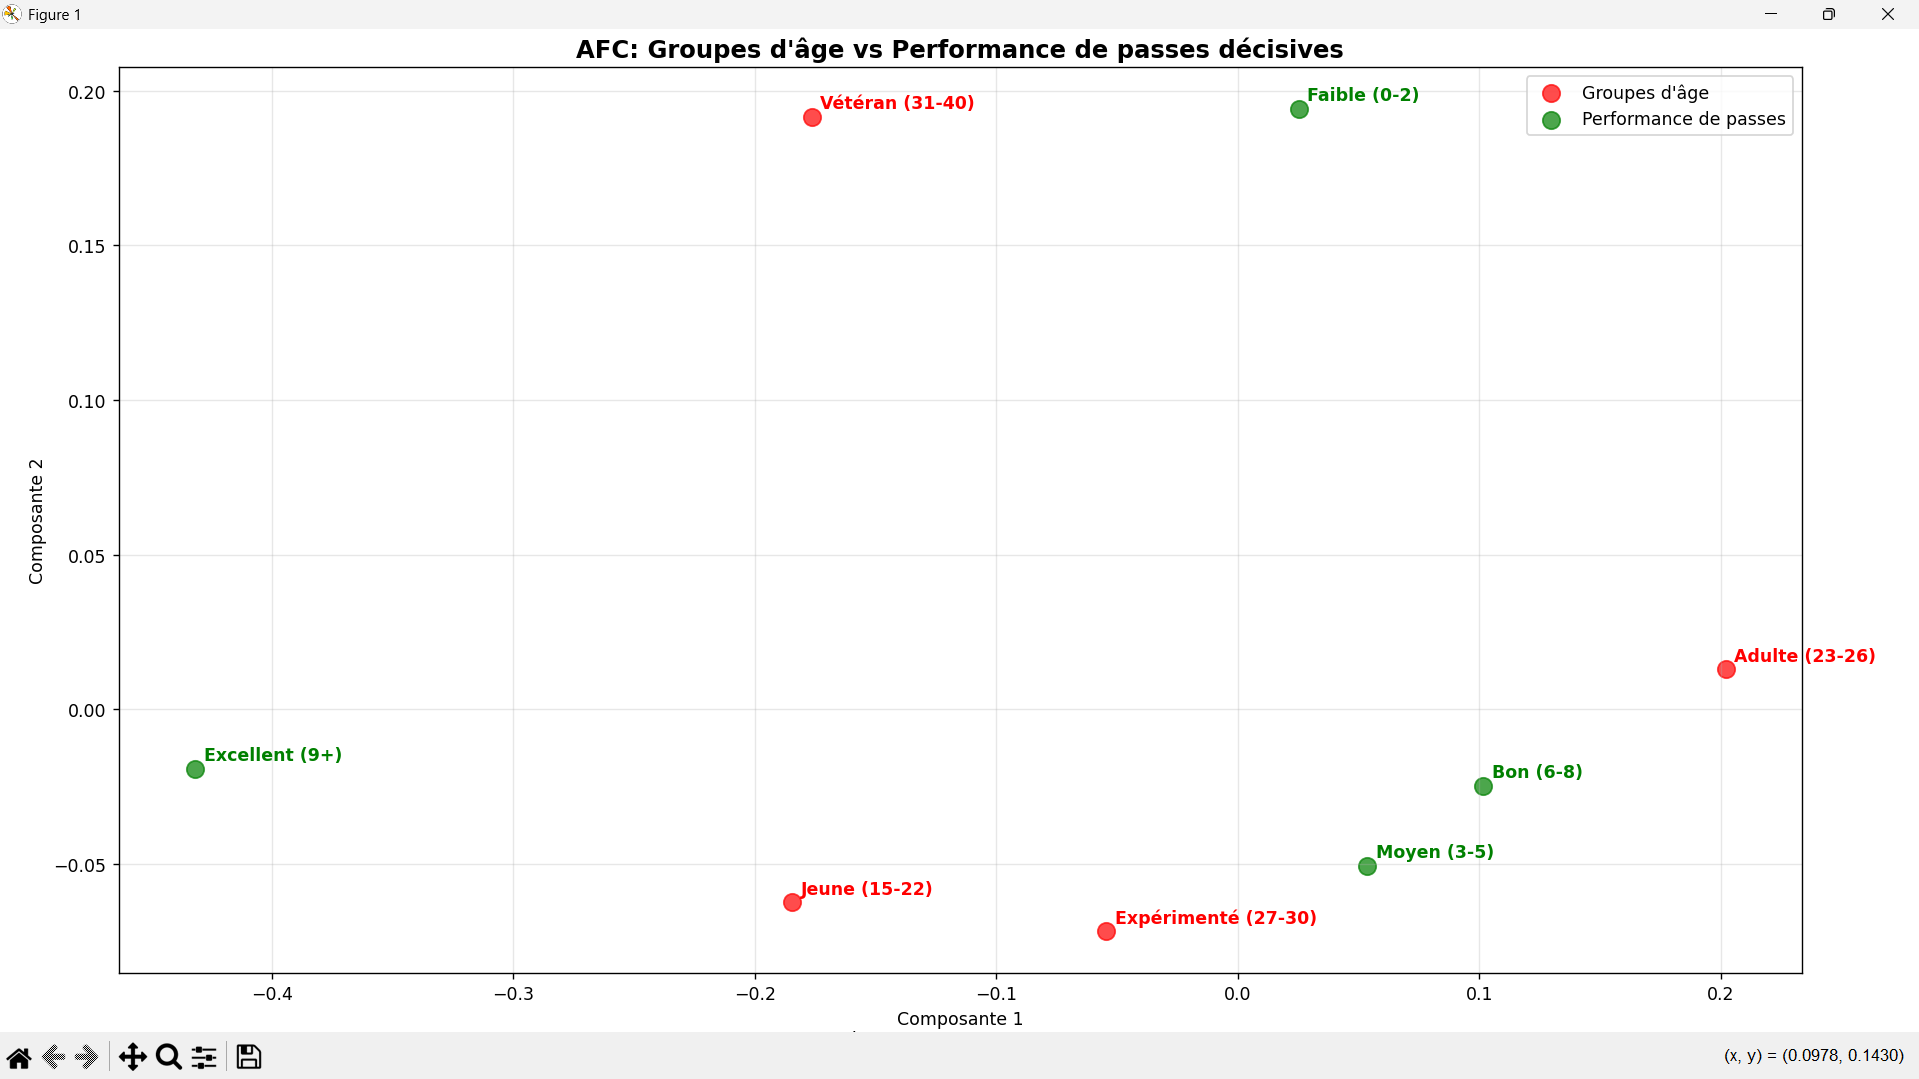
\includegraphics[width=1\textwidth]{images/graphique_AFC_passes.png}
                    \captionof{figure}{}
                \end{center}

            \subsubsection{Interprétation}
                Dans la figure ci-desssus, on peut observer une évidente structure claire entre les groupes d’âge et la performance en passes décisives. En effet, on observe que les jeunes (15–22 ans) et les joueurs expérimentés (27–30 ans) sont situés du même côté que la catégorie "Excellent (9+)", ce qui indique une forte association entre ces tranches d’âge et les meilleures performances en termes de passes décisives. Ces résultats suggèrent que la créativité et la vision du jeu, essentielles à la réussite des passes, sont particulièrement marquées chez les joueurs jeunes et expérimentés. En d'autres termes, on peut affirmer qu'ils sont à leur prime (le sommet de leurs performances).\\\\
                À l’inverse, les adultes (23–26 ans) se rapprochent des modalités "Bon (6–8)" et "Moyen (3–5)", traduisant des performances solides mais moins marquantes, tandis que les vétérans (31–40 ans) se trouvent à proximité de la catégorie "Faible (0–2)", indiquant un déclin des performances avec l’âge.


    %%%%%%%%%%%%%%%%%%%%%%%%%%%%%%%%%%%%%%%%%%%%%%%%%%%%%%%%%%%%%%%%%%%%%%%%%%%%%%%%%%%
    %%%%%%%%%%                      ANALYSE MIXTE : ACM                      %%%%%%%%%%
    %%%%%%%%%%%%%%%%%%%%%%%%%%%%%%%%%%%%%%%%%%%%%%%%%%%%%%%%%%%%%%%%%%%%%%%%%%%%%%%%%%%

    \section{Analyse mixte des données : ACM}

        \subsection{Définition}
            L'Analyse des Correspondances Multiples (ACM) est une technique statistique utilisée pour analyser des données qualitatives comportant plusieurs variables. Elle permet de représenter graphiquement les relations entre les différentes catégories des variables, en les projetant dans un espace à deux dimensions.\\\\
            L'ACM est particulièrement utile pour identifier des associations entre les catégories, détecter des groupes similaires et comprendre la structure sous-jacente des données qualitatives. En réduisant la complexité des données, l'ACM facilite l'interprétation et la communication des résultats.

        \subsection{Graphique des modalités}
            
            \subsubsection{Définition}
                Le graphique des modalités est un outil visuel utilisé dans le cadre de l'ACM pour représenter les relations entre les catégories de plusieurs variables qualitatives. Chaque catégorie est représentée par un point dans un plan défini par les deux premières dimensions de l'analyse.\\\\
                Ce graphique permet d'identifier des associations entre les catégories, des tendances générales, ainsi que des groupes similaires. En analysant la distribution des points, on peut tirer des conclusions sur la structure sous-jacente des données et sur les relations entre les différentes catégories.\\

                \begin{center}
                    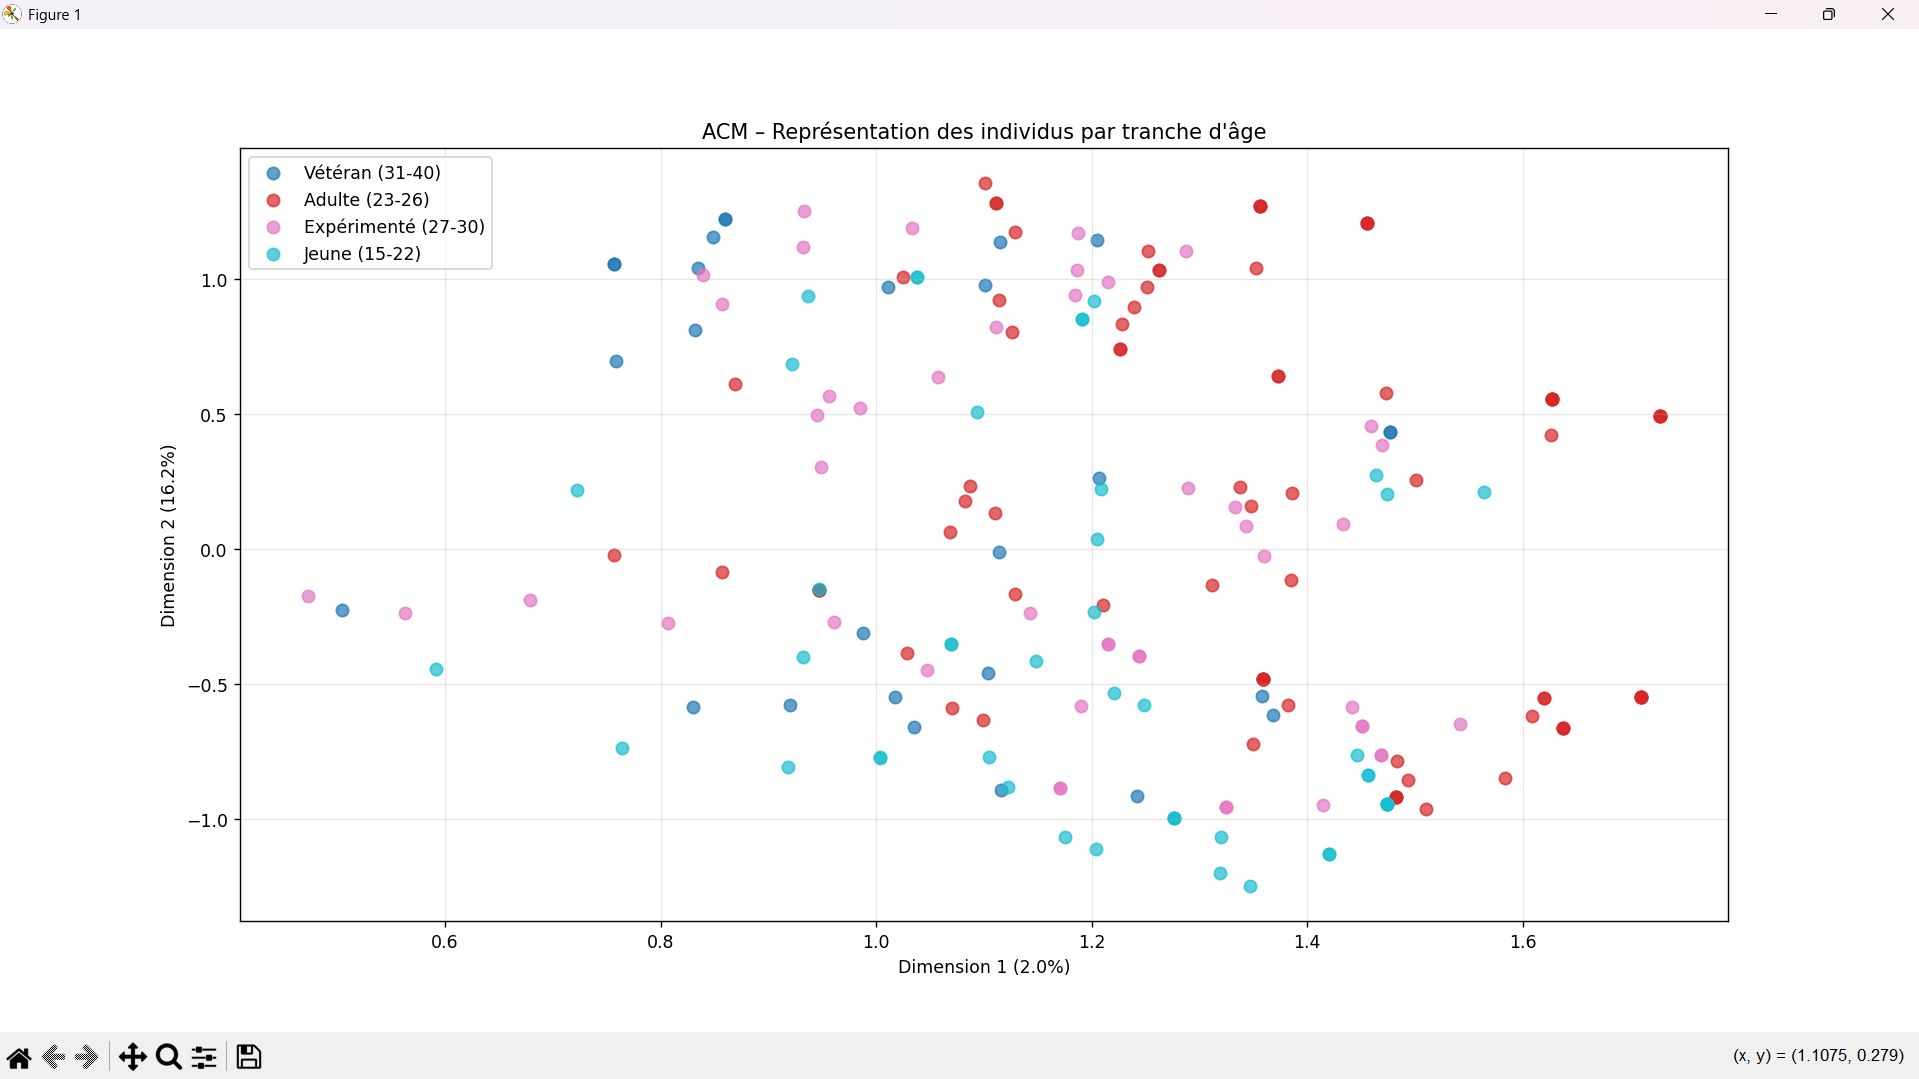
\includegraphics[width=1\textwidth]{images/graphique_ACM_ages.png}
                    \captionof{figure}{}
                \end{center}

        \subsubsection{Interprétation}
                Dans la figure ci-dessus, on peut observer que les jeunes (15-22 ans) sont situés sur la partie inférieure du graphique, signifiant qu'ils ont tendance à être beaucoup moins performant que les joueurs adultes (23-26 ans) et expérimentés (27-30 ans) qui eux, sont situés dans la partie supérieure du graphique indiquant donc de meilleures performances en général.\\\\
                Les vétérans (31-40 ans) eux, sont répartis équitablement sur le graphique (environ 50\% dans la partie positive de la deuxième dimension et environ 50\% dans la partie négative de cette même dimension), ce qui suggère que certains vétérans parviennent à maintenir des performances élevées malgré leur âge avancé, tandis que d'autres connaissent un déclin plus marqué.\\


    %%%%%%%%%%%%%%%%%%%%%%%%%%%%%%%%%%%%%%%%%%%%%%%%%%%%%%%%%%%%%%%%%%%%%%%%%%%%%%%%%%%
    %%%%%%%%%%                            CONCLUSION                         %%%%%%%%%%
    %%%%%%%%%%%%%%%%%%%%%%%%%%%%%%%%%%%%%%%%%%%%%%%%%%%%%%%%%%%%%%%%%%%%%%%%%%%%%%%%%%%

    \section{Conclusion}

        En conclusion, notre analyse des données des joueurs de football évoluant dans les cinq meilleures ligues européennes durant la saison 2024-2025 a permis de mettre en lumière plusieurs aspects intéressants. L'ACP a révélé des groupes distincts de joueurs basés sur leurs performances statistiques, tandis que l'AFC a montré des associations claires entre l'âge des joueurs et leurs performances en termes de buts et de passes décisives. Enfin, l'ACM a permis d'identifier des tendances générales concernant les performances en fonction de l'âge.\\\\
        Ces analyses fournissent une compréhension approfondie des dynamiques du football professionnel et peuvent être utiles pour les entraîneurs, les recruteurs et les analystes sportifs dans leurs prises de décisions. Pour des analyses futures, il serait intéressant d'intégrer davantage de variables qualitatives, quantitatives ainsi que de joueus et d'examiner les performances sur plusieurs saisons pour observer les tendances à long terme.\\


\end{document}